\begin{figure}[htbp]
    \centering
    \definecolor{waterblue}{RGB}{65,190,225}
    \definecolor{mercurygray}{RGB}{105,105,105}
    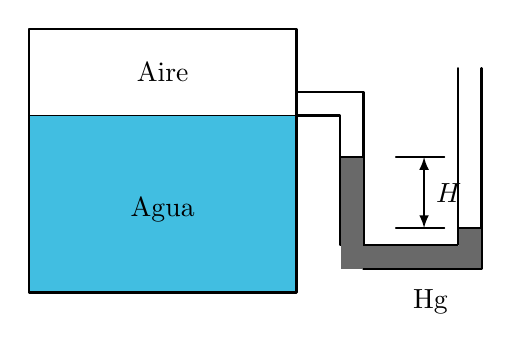
\begin{tikzpicture}[x=1cm,y=1cm,line cap=round,line join=round]
        % Depósito cerrado
        \fill[waterblue] (0,0) rectangle (3.4,2.25);
        \draw[line width=0.8pt] (0,0) rectangle (3.4,3.35);
        \draw[line width=0.5pt] (0,2.25) -- (3.4,2.25);
        \node at (1.7,2.80) {Aire};
        \node at (1.7,1.05) {Agua};

        % Tubería que conecta el depósito con el manómetro
        \draw[line width=0.8pt]
            (3.4,2.55) -- (4.25,2.55) -- (4.25,0.30)
            -- (5.75,0.30) -- (5.75,2.85);
        \draw[line width=0.8pt]
            (3.4,2.25) -- (3.95,2.25) -- (3.95,0.60)
            -- (5.45,0.60) -- (5.45,2.85);

        % Mercurio en el tubo en U
        \fill[mercurygray]
            (3.96,0.30) -- (4.24,0.30) -- (4.24,1.72)
            -- (3.96,1.72) -- cycle;
        \fill[mercurygray] (4.24,0.31) rectangle (5.46,0.59);
        \fill[mercurygray] (5.46,0.31) rectangle (5.74,0.82);

        % Superficies de separación
        \draw[line width=0.5pt] (3.96,1.72) -- (4.24,1.72);
        \draw[line width=0.5pt] (5.46,0.82) -- (5.74,0.82);

        % Cota H entre los niveles del mercurio
        \draw[latex-latex,line width=0.6pt] (5.02,0.82) -- (5.02,1.72);
        \draw[line width=0.5pt] (4.66,0.82) -- (5.28,0.82);
        \draw[line width=0.5pt] (4.66,1.72) -- (5.28,1.72);
        \node[right] at (5.05,1.27) {$H$};

        \node at (5.10,-0.12) {Hg};
    \end{tikzpicture}
    \caption{Manómetro del problema 2.}
\end{figure}
